\chapter{実験}\label{sec:Experiments}
ここでは,いくつかの予備実験の結果を示したのちに,提案手法を先行研究と比較した結果を示し,考察を行う.

%%%%
\section{予備実験}\label{sec:PreExperiments}
提案手法の妥当性を確認するため,2点の改良点をもとにアブレーション実験を実施した.

%%%%
\subsection{データセットによる比較}\label{sec:PreEx_Dataset}

%%%%
\subsection{バッチサイズによる比較}\label{sec:PreEx_Batchsize}

%%%%
\subsection{予備実験の考察}\label{sec:PreEx_consideration}

%%%%
\section{実験}\label{sec:Experiment} % 本当は章と節で同じタイトルにするのはふさわしくない.また,全く同じラベルは指定できない(指定すると上書きされる)

ここでは,先行研究として~~の手法\cite{ref:yao2017integrated}および~~の手法\cite{ref:nomura2022uwb}を取り上げ,提案手法との比較及び考察を実施する.
実験環境を表\ref{tab:ExEnvironment}に示す.

\begin{table}[htbp]
    \centering
    \input{table/ExEnvironment.txt} % 表本体が記されたテキストファイル
    \caption{実験環境} % 表の題名
    \label{tab:ExEnvironment} % 表のラベル(tab:から始めるとわかりやすい)
\end{table}

損失をグラフ化したものを図\ref{fig:LossGraph}に示す.図\ref{fig:LossGraph}より,~~

また,図\ref{fig:Result}に2種類のデータについて入力画像と出力画像を並べた結果を示す.図\ref{fig:Result_1}では~~であるのに対して,図\ref{fig:Result_2}では~~

\begin{figure}[htbp]
    \centering
    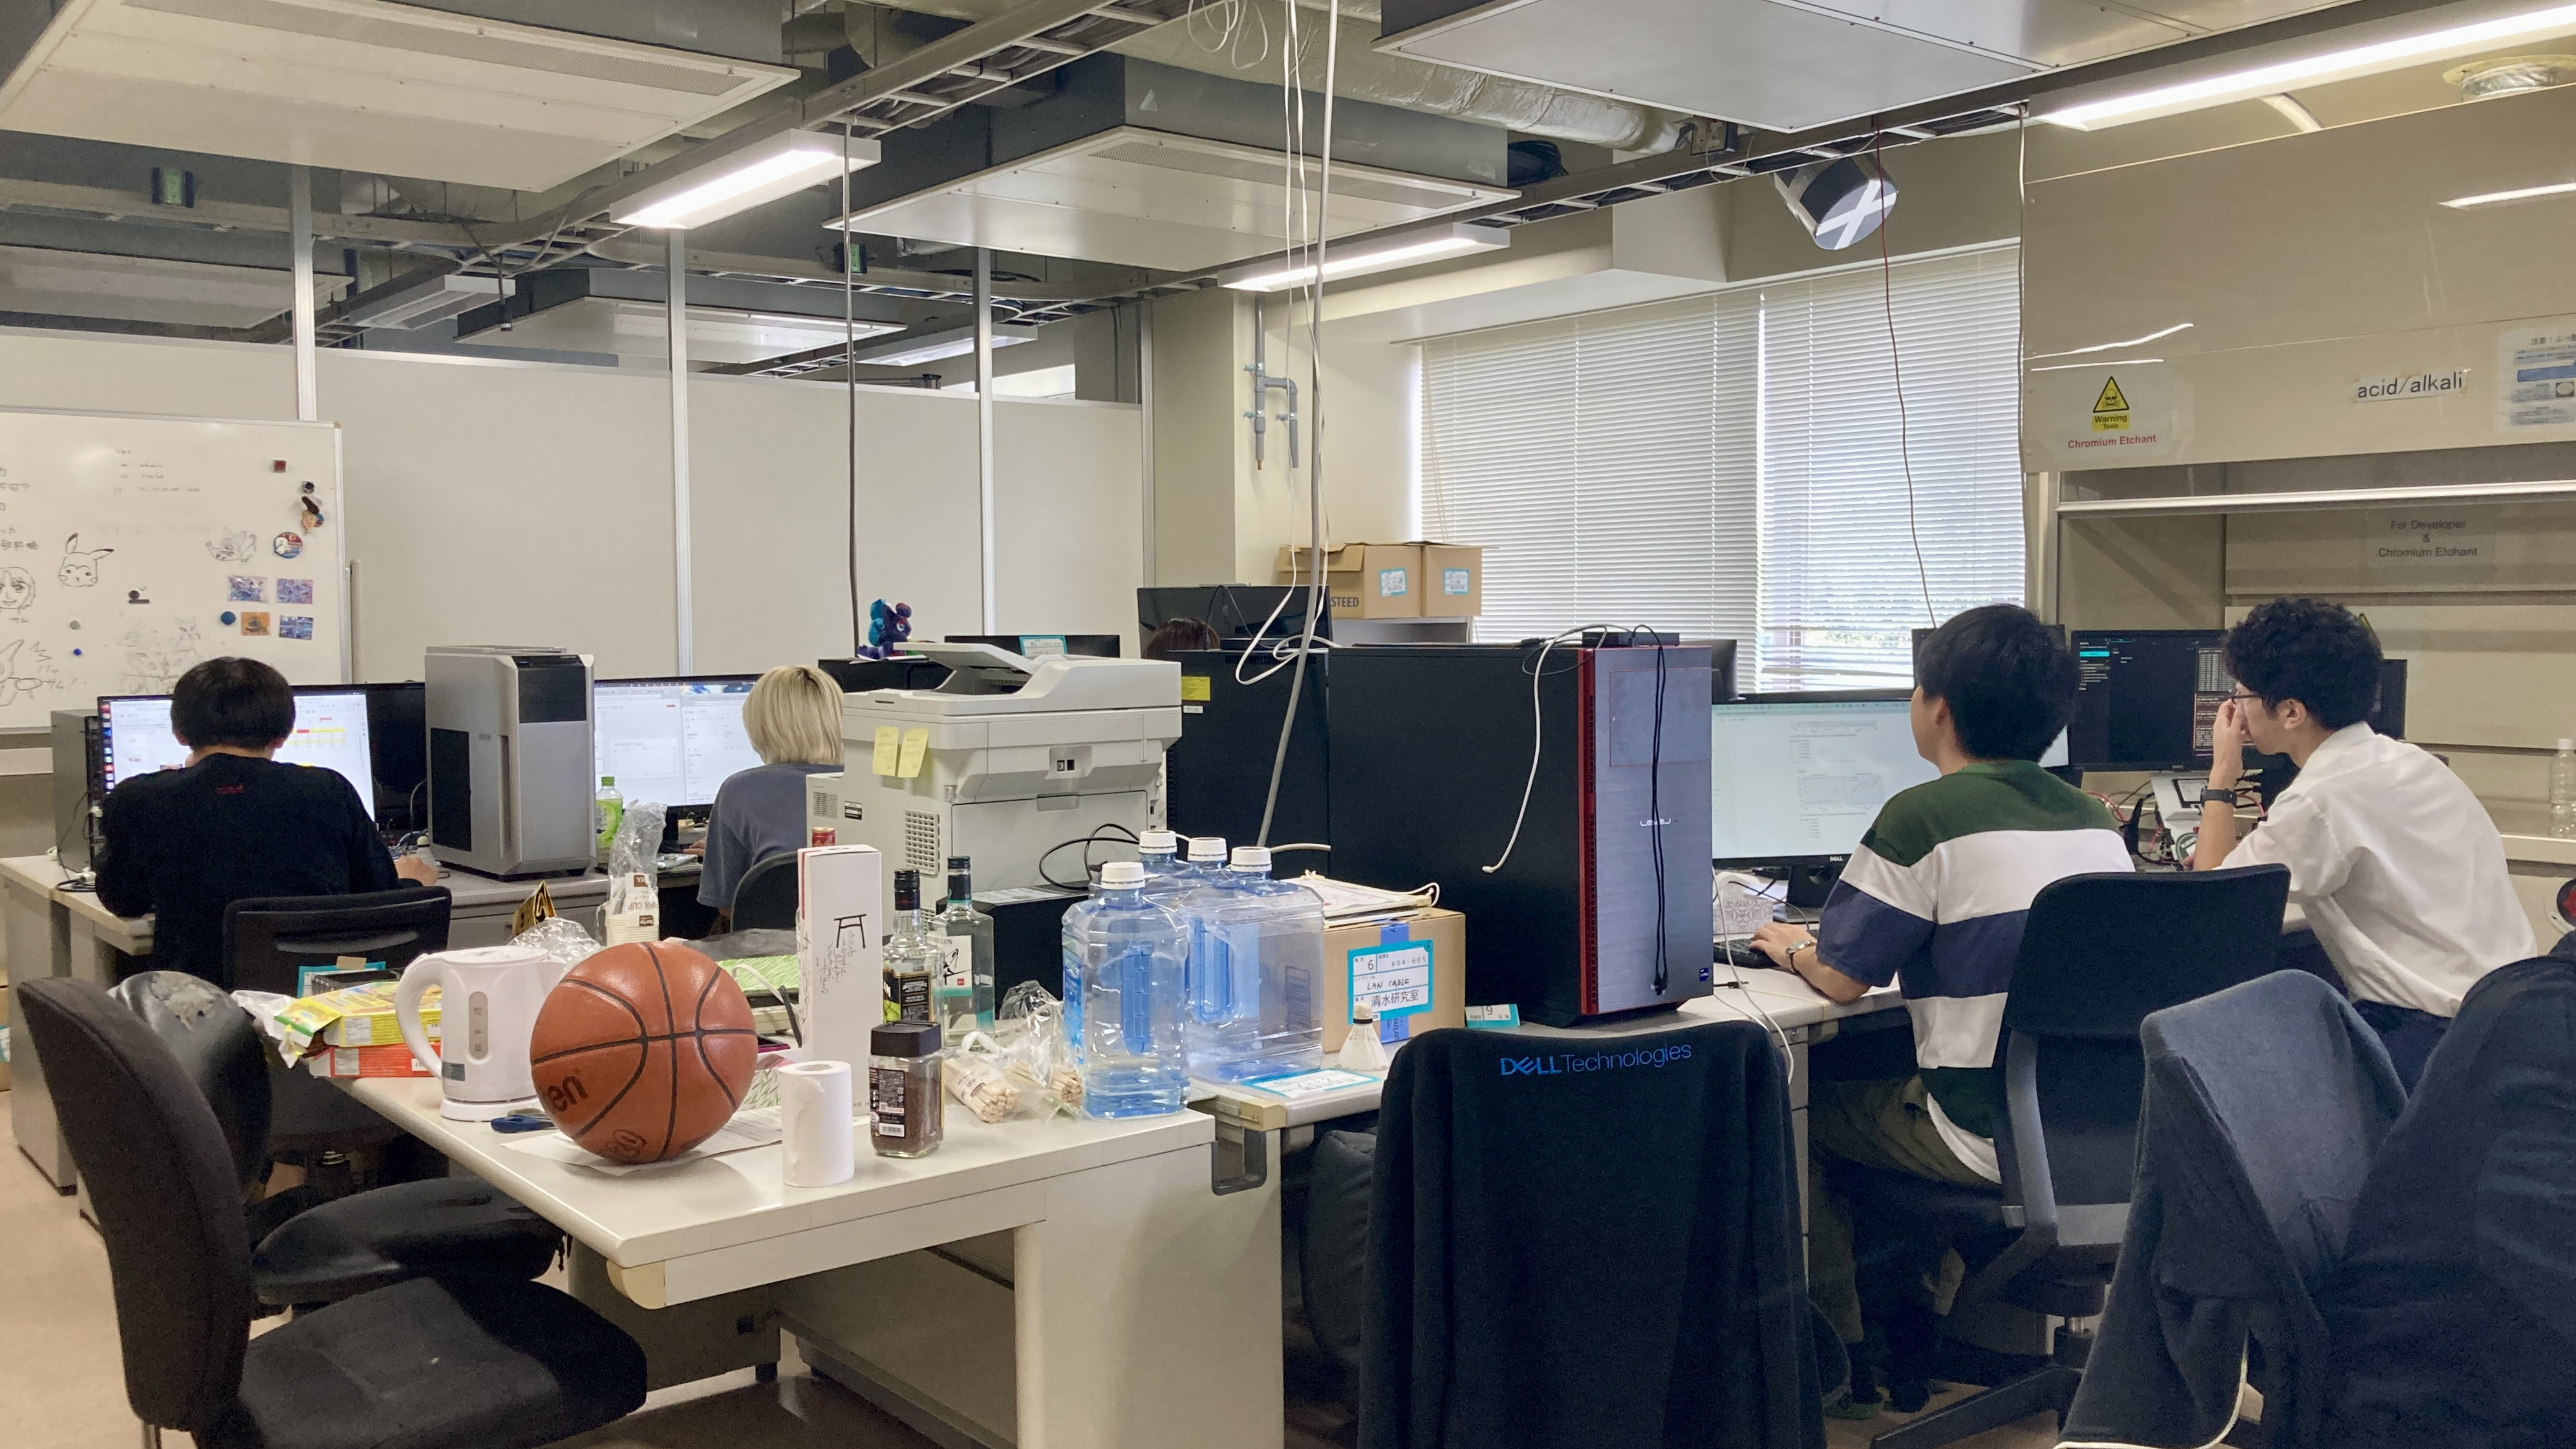
\includegraphics[width=.5\textwidth]{figure/labpic.jpg} % 紙面の横幅の0.5倍で図を挿入する
    \caption{損失} % 図の題名
    \label{fig:LossGraph} % 図のラベル(fig:から始めるとわかりやすい)
\end{figure}

\begin{figure}[H]
	\begin{minipage}{.5\textwidth}
        \centering
		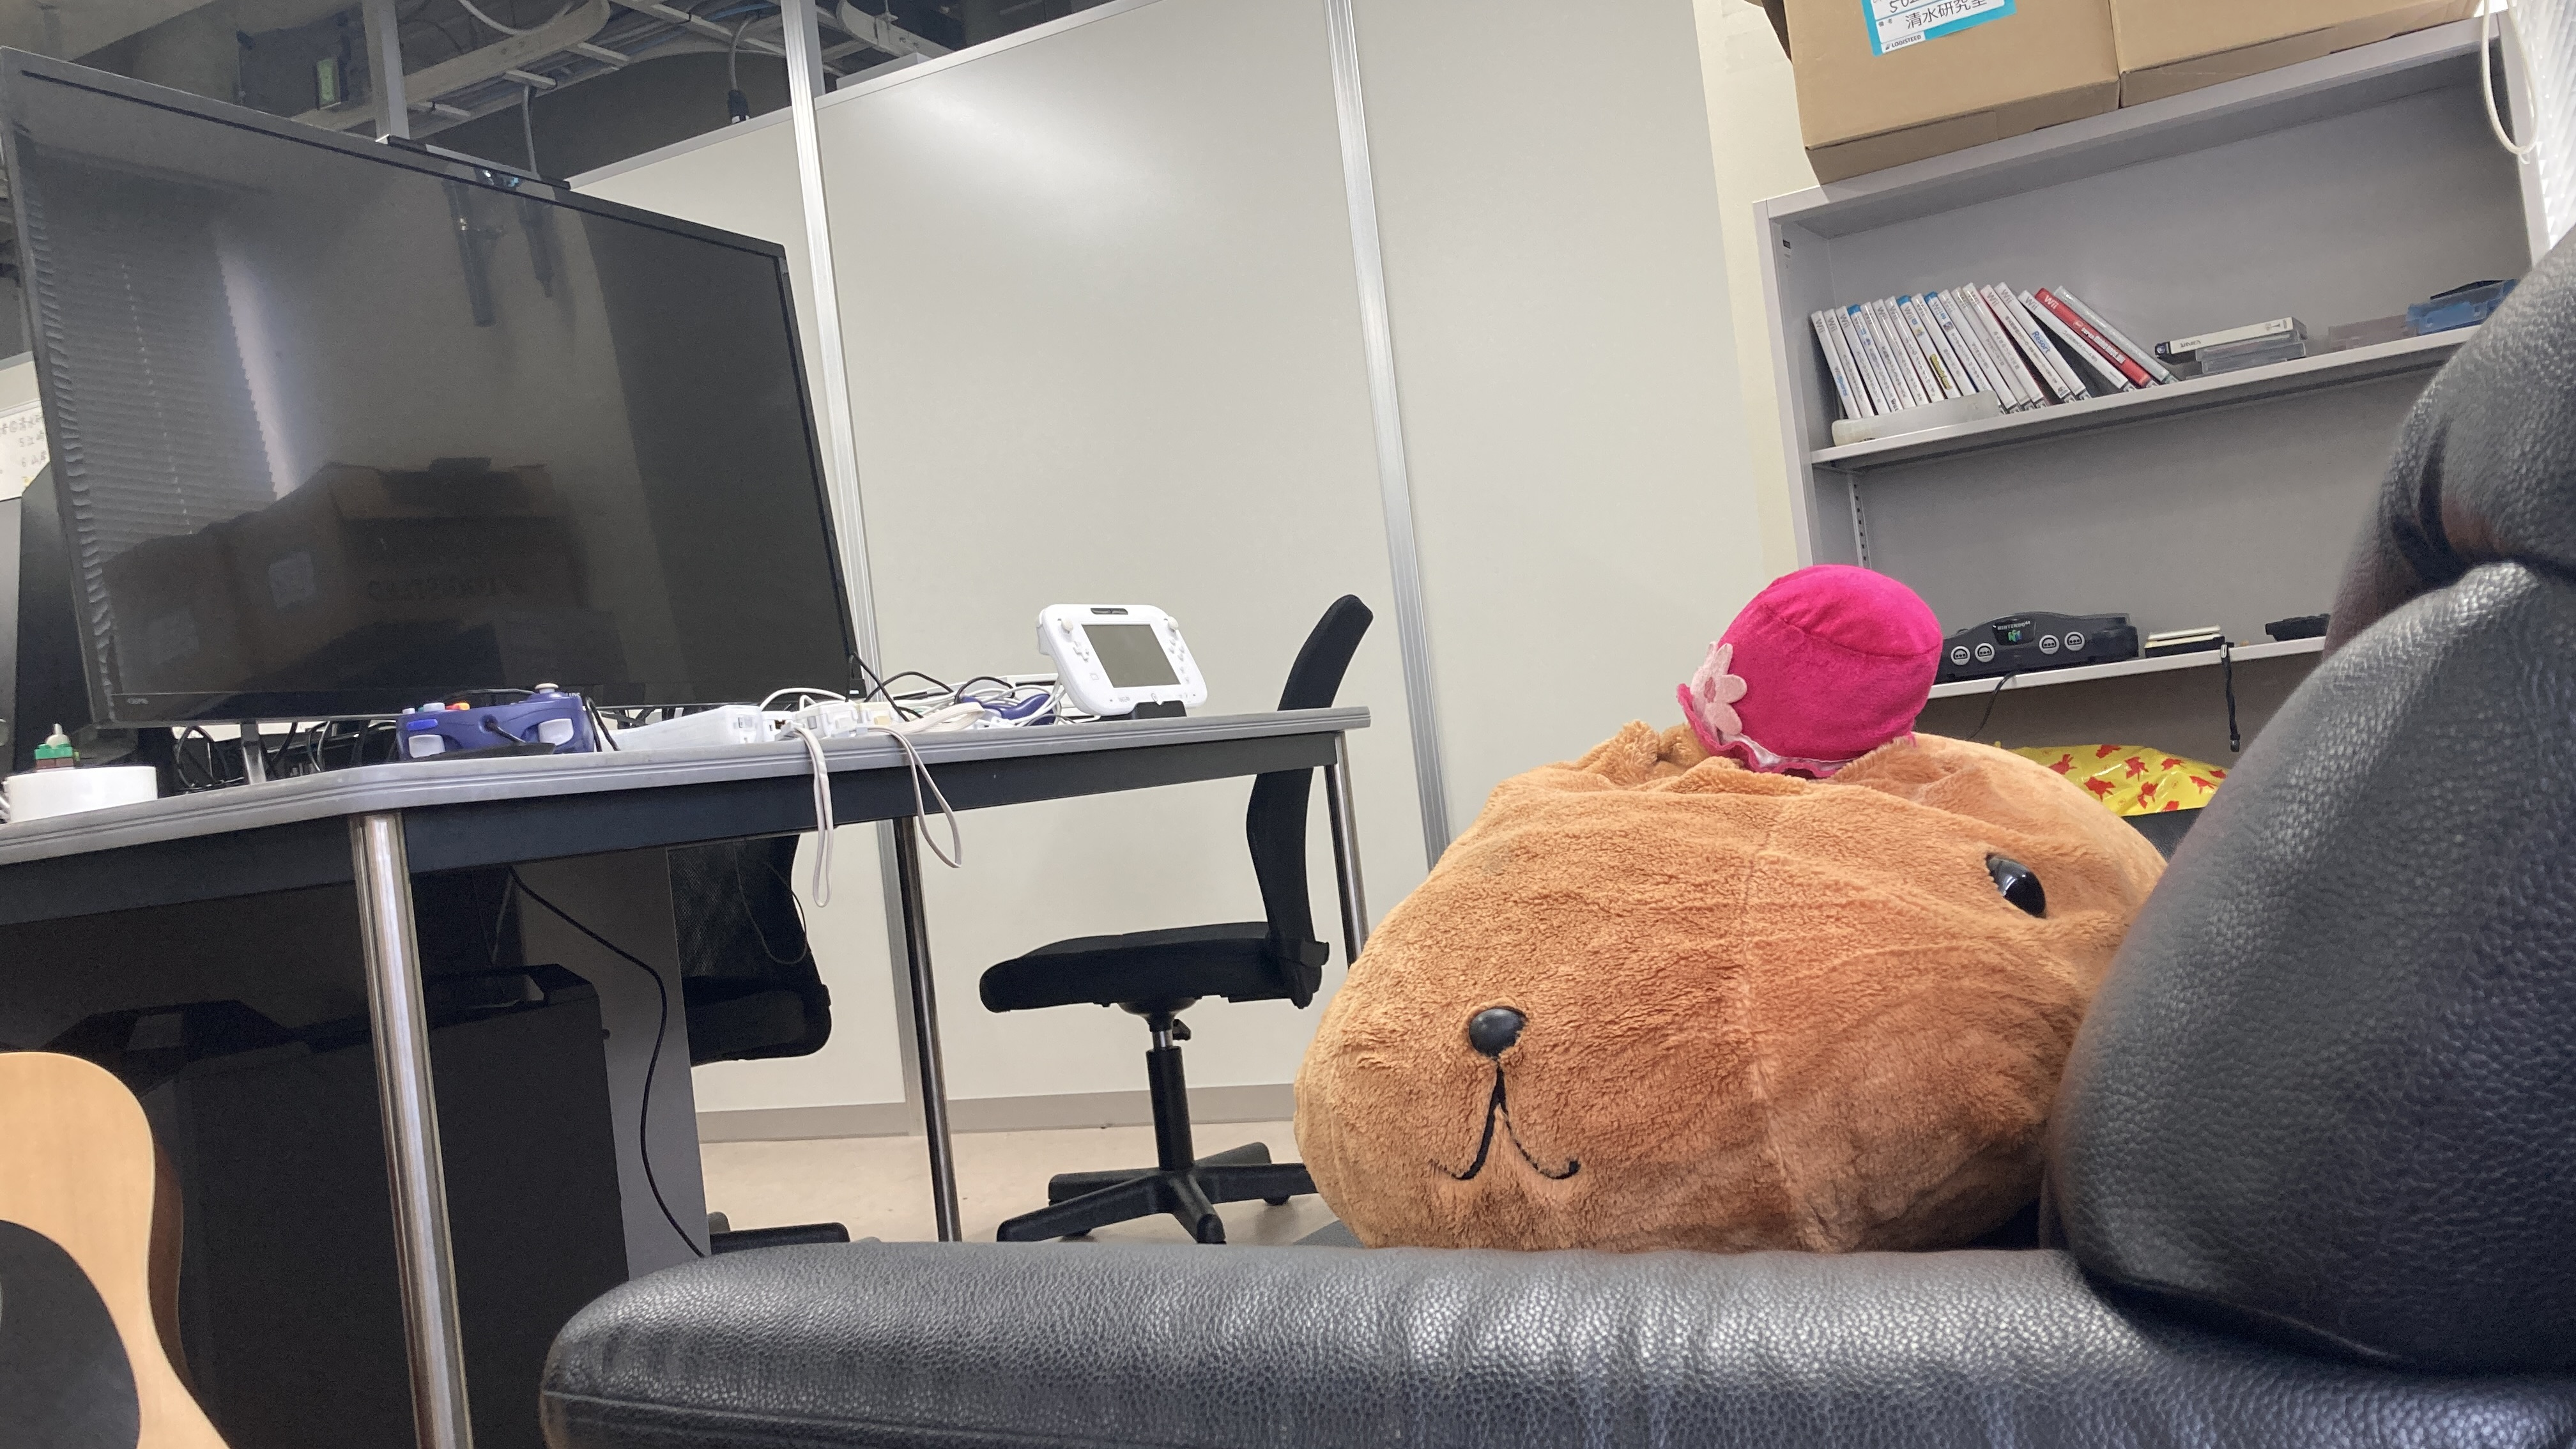
\includegraphics[width=.95\textwidth]{figure/labpic_game.jpg}
		\subcaption{入力画像(1)と出力の様子} % subcaptionを使うことで図1(a)のような表記が可能.使いたくなければcaptionに変更する
        \label{fig:Result_1}
	\end{minipage}\hfill
 	\begin{minipage}{.5\textwidth}
        \centering
		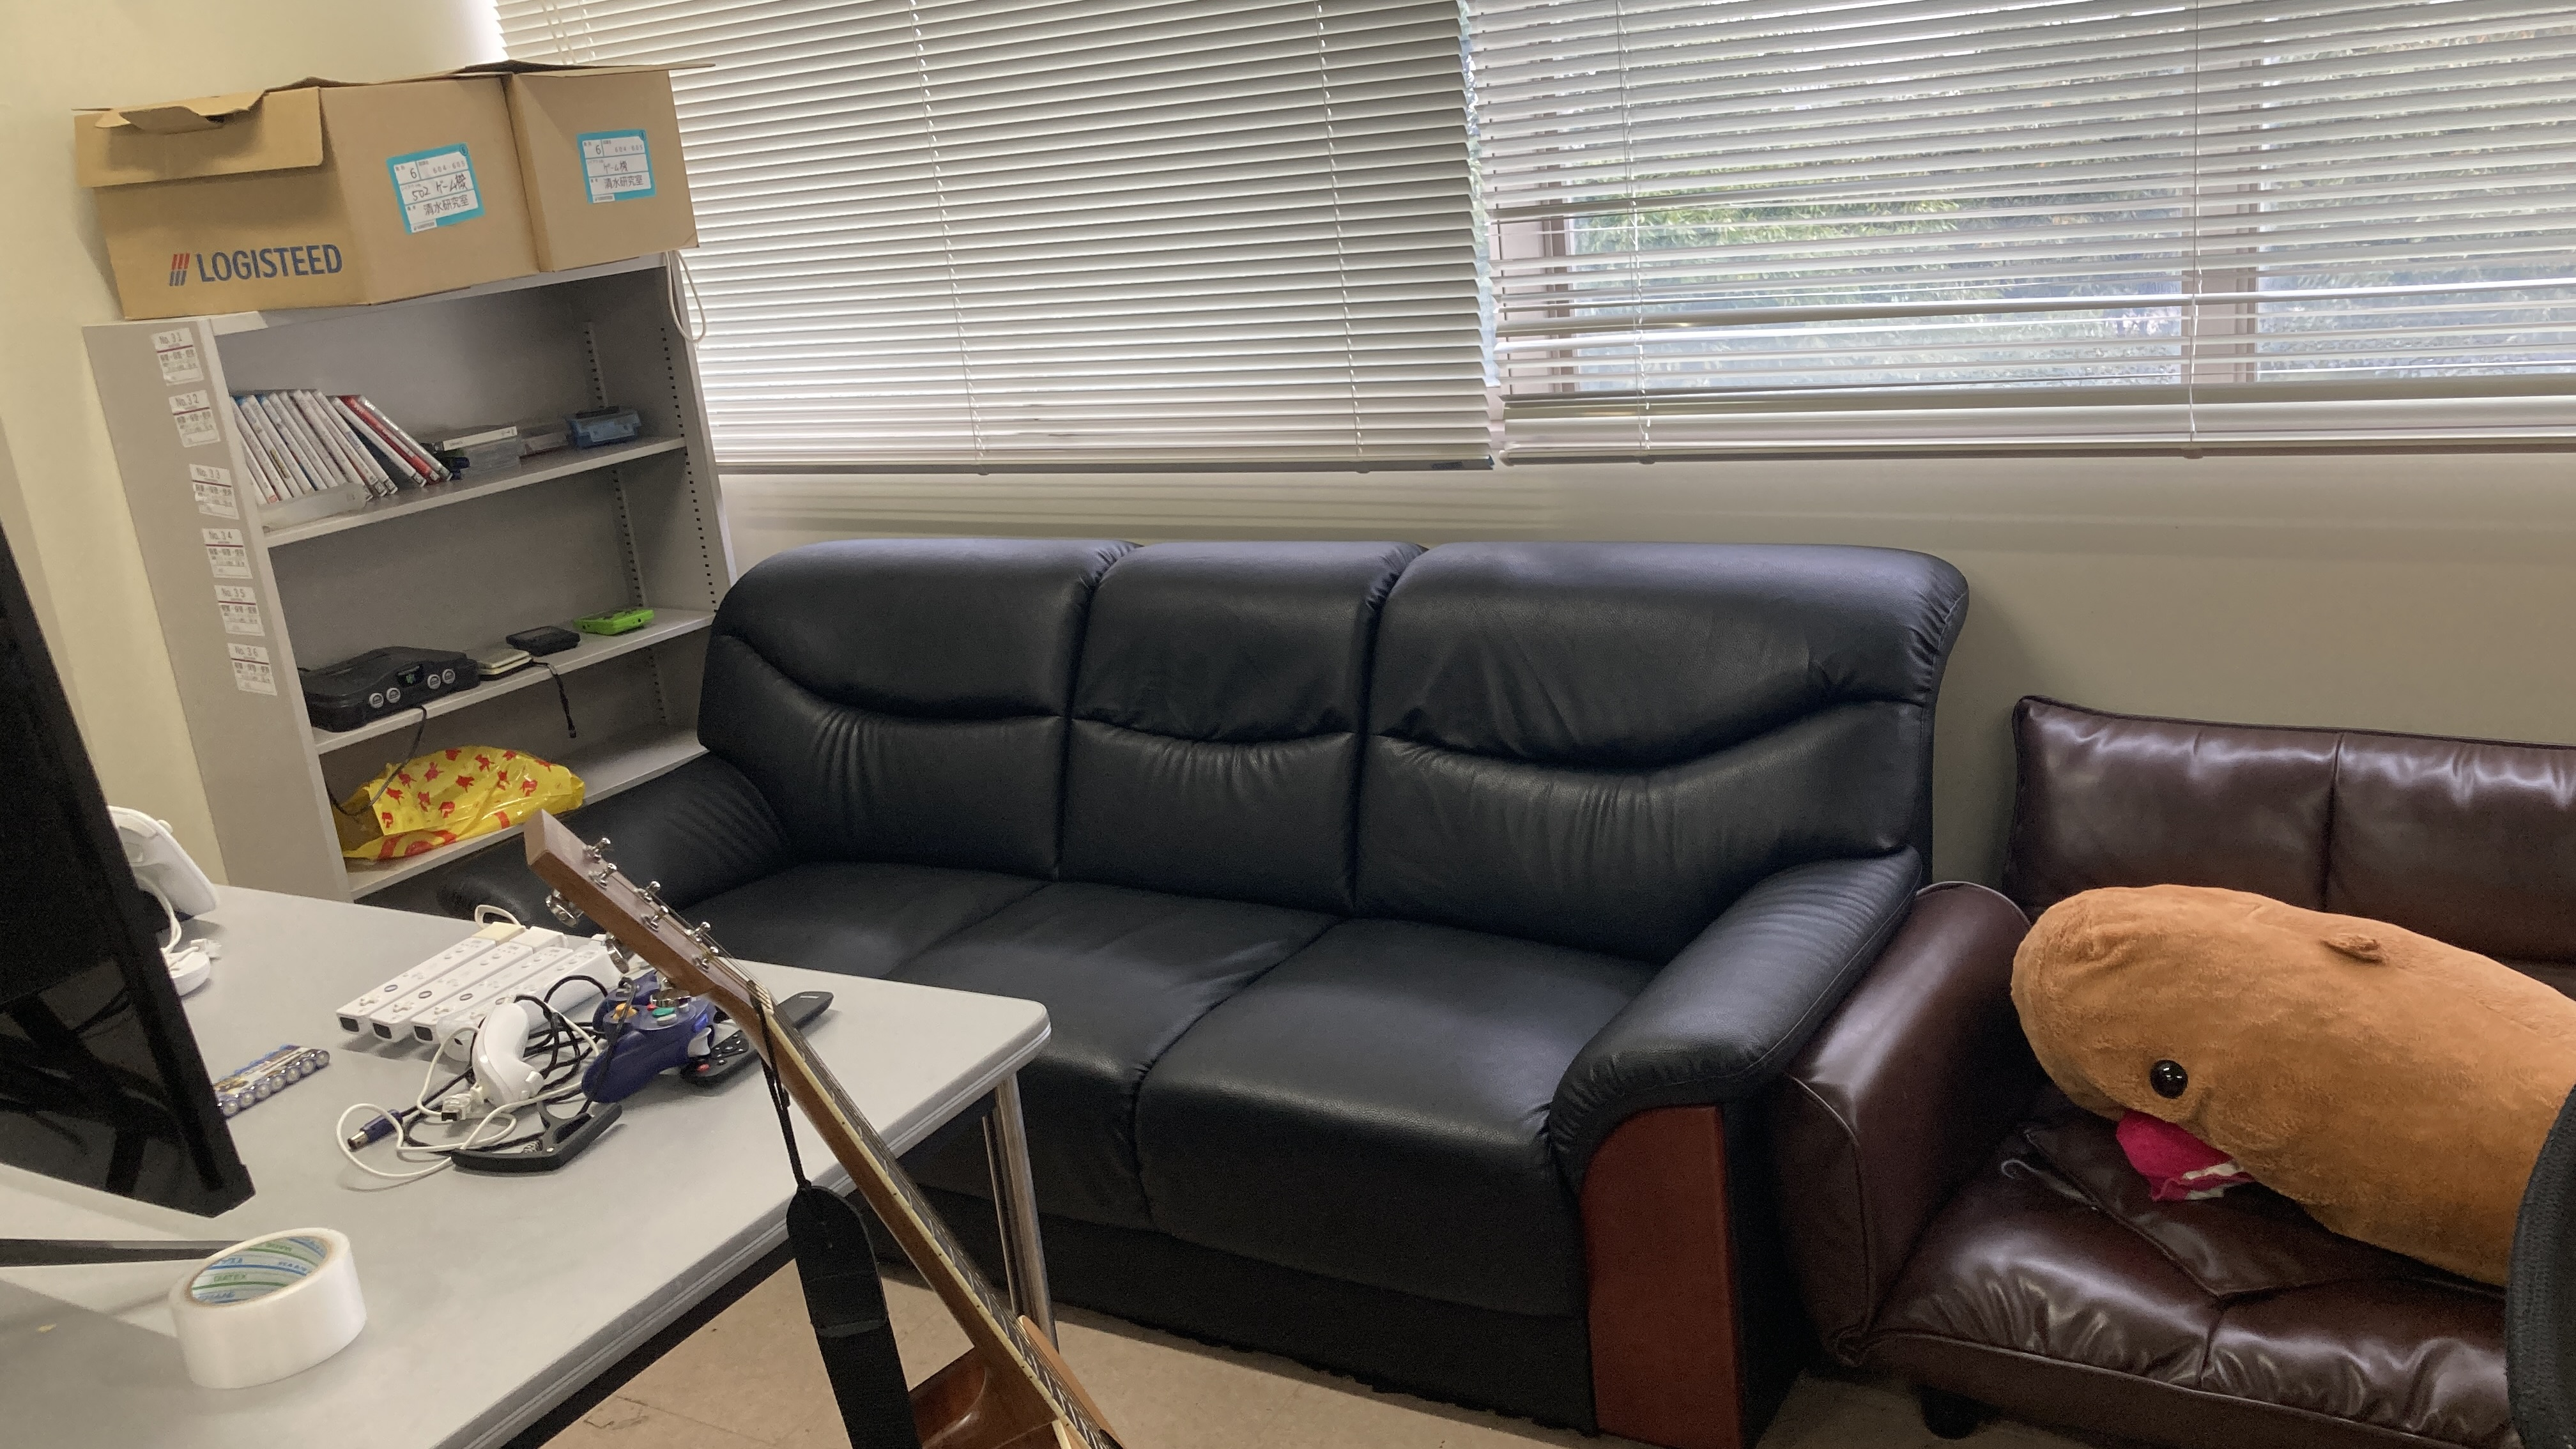
\includegraphics[width=.95\textwidth]{figure/labpic_sofa.jpg}
		\subcaption{入力画像(2)と出力の様子}
        \label{fig:Result_2}
	\end{minipage}\hfill
	\caption{入力画像と出力の様子}\label{fig:Result}
\end{figure}


%%%%
\subsection{考察}\label{sec:Ex_consideration}
